\documentclass[a4]{MScthesis}
\usepackage{parskip}
\setlength{\parindent}{0cm}
\usepackage{ae}
\usepackage{pdfpages}
\usepackage{booktabs}
\usepackage{varioref}
\usepackage{natbib}
\usepackage{siunitx}
\usepackage{hyperref}
\usepackage{todonotes}
\usepackage{graphicx}
\usepackage{subfig}
\usepackage{rotating}
\usepackage{caption}
\usepackage{tablefootnote}

\usepackage{tikz}
\usetikzlibrary{patterns}


\title{Camera-assisted ROV navigation in sea cages} % The title of your assignement; NB use \newlinetitle to start a newline
\author{Morten Engelhardt Olsen} % Your firstname and lastname
\professor{Jo Arve Alfredsen, ITK} % Affiliation = ITEM for instance
\supervisor{Jo Arve Alfredsen, ITK\\ & Per Rundtop, SINTEF Fiskeri og Havbruk}

%% Uncomment the following in case you want subfigures; note that there will be a warning for the caption package
% \let\subcaption\undefined
% \let\subfloat\undefined
% \usepackage[bf]{caption}
% \usepackage{subcaption}

\DeclareGraphicsExtensions{.pdf,.jpg,.png}
\graphicspath{{./figs/}}

%\loadglsentries{glossary}
%\makeglossaries

\begin{document}
\selectlanguage{english}
\pagenumbering{roman}
\pagestyle{plain}

%% Only for the project
\titleITEM

\cleardoublepage
\includepdf[pages={1}]{assig.pdf}
\cleardoublepage
%% Only for the master's thesis; for the project report the description is taken from It's Learning and added by the department
% \selectlanguage{english} % Change to 'norsk' if you are writing in Norwegian
% \input{problem_description}
% \cleardoublepage

%% There must be an abstract in English, even though the main text is in Norwegian
\selectlanguage{english}
\begin{abstract}
This thesis is a preliminary study of the feasibility of using 
modern computer vision algorithms for navigation in specific 
and known underwater environments. Using new high definition camera 
technologies and .... \todo{MORE}
\end{abstract}
\cleardoublepage

%% Only for the master's thesis; if the main text is in English and you can write Norwegian, there must be an abstract in Norwegian as well.A
% \selectlanguage{norsk}
% \include{abstract_norwegian}
% \cleardoublepage

\selectlanguage{english}% Change to 'norsk' if you are writing in Norwegian

%
\chapter{Preface}


\section{Acknowledgements}

I would like to thank Terje Haugen (ITK) at the departments mechanical workshop for 
helping with design and the actual making of the underwater housing for the test system.

A thank also goes to Kevin Frank (SINTEF) and Per Rundtop (SINTEF) for expertise 
in aquaculture and use of their test rig and cooperation in the field testing. 

A special thanks goes to Trond Viggo Melum (NRK) for help with troubleshooting the HD-SDI interface.

Thanks to Rolf Hansen (Malvik småbåtforening) for lending some space in the harbour for the rigging.

And last but not least, a big thank to Jo Arve Alfredsen (ITK) for support and 
brilliant guidance during the rougher times of this thesis.
\cleardoublepage

% similarly you may add a separate acknowledgments page

\tableofcontents*
\cleardoublepage

%% include if relevant
\listoffigures
\cleardoublepage

%% include if relevant
\listoftables
\cleardoublepage

%% include if relevant
%\listofalgorithms
%\addcontentsline{toc}{chapter}{List of Algorithms}
%\cleardoublepage

%% include if relevant
%\printglossary[title=List of Symbols, style=long]
%\cleardoublepage
%\glsaddall[]

%% include if relevant
%\printglossary[title=List of Acronyms,type=\acronymtype] % prints just the list of acronyms
%\cleardoublepage

\pagenumbering{arabic}
\pagestyle{ruled}



\chapter{Preface}


\section{Acknowledgements}

I would like to thank Terje Haugen (ITK) at the departments mechanical workshop for 
helping with design and the actual making of the underwater housing for the test system.

A thank also goes to Kevin Frank (SINTEF) and Per Rundtop (SINTEF) for expertise 
in aquaculture and use of their test rig and cooperation in the field testing. 

A special thanks goes to Trond Viggo Melum (NRK) for help with troubleshooting the HD-SDI interface.

Thanks to Rolf Hansen (Malvik småbåtforening) for lending some space in the harbour for the rigging.

And last but not least, a big thank to Jo Arve Alfredsen (ITK) for support and 
brilliant guidance during the rougher times of this thesis.
\cleardoublepage{}


\chapter{Introduction}
During the last four decades, the demand for fish 
has been steadily increasing. The current level 
of demand supersedes the amount of fish that 
can be fished and keep the different stocks of 
fish at a sustainable level. This has lead to 
overfishing, eliminating for instance the 
fish population on the Grand Banks off the east 
coast of America. Many other fish 
populations are also either gone or in fast 
diminish. Some scientists are even predicting 
that with the current overfishing, the fish industry will 
see a global collapse during this century \citet{worm06}.

To combat the overfishing of natural fish stocks are to increase 
the production of fish through farming. This way of ensuring 
sustainability for both stocks and people has been 
used for millenias on land, and is now being rapidly 
deployed on sea. According to \citet{fao06}, the amount of 
fish that were farmed globally in 2005 was 48.1 million tons, out of 
a total 141.3 million tons of fish that were produced. This 
means that about a third of all fish sold were farmed in 2005, with 
steadily increasing numbers.




\section{Motivation}


\section{Previous Work}


\section{Outline}


\cleardoublepage{}


\chapter{Specification}


\section{Hardware}

\subsection{Argus hardware}

\subsection{High definition video hardware}

\subsection{High definition video signalling}

\section{Software}

\subsection{High definition video capture}

\subsection{High definition video analysis}

\subsection{Real time constraints}


\cleardoublepage{}



\chapter{Laser-based Orientation}
In this...

\section{Projections}
The use of some regular and known geometrical shape that could be projected onto the net for use for orientation 
was early put forward. The idea behind this is based on the work by \citet{carlsen10}, who used 
a set of line lasers for \todo{Hva var dette egentlig?}

\section{Patterns}
There are many different patterns that may give more information about 
orientation of the ROV relative to the net than some simple lines. The 
different polygons in figure \vref{fig:pattern_triangle} to \vref{fig:pattern_heptagon}
were chosen as a good start for further investigation together with the 
circle as shown in \vref{fig:pattern_circle}.

\begin{figure}[htbp]
	\subfloat[Triangle]{
		
\begin{tikzpicture}[scale=0.1]
			\draw (0,4) -- (11,15) -- (15,0) -- (0,4);
		\end{tikzpicture}\label{fig:pattern_triangle}
	}\hfill
	\subfloat[Square]{
		\begin{tikzpicture}[scale=0.1]
			\draw (0,0) -- (0,15) -- (15,15) -- (15,0) -- (0,0);
		\end{tikzpicture}
	}\hfill
	\subfloat[Pentagon]{
		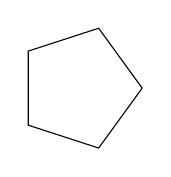
\begin{tikzpicture}[scale=1]
			\newdimen\R
			\R=0.8cm
			\draw (0:\R)
				\foreach \x in {72,144,...,360} {  -- (\x:\R) };
		\end{tikzpicture}
	}\hfill
	\subfloat[Hexagon]{
		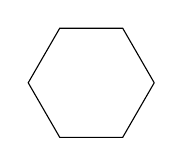
\begin{tikzpicture}[scale=1]
			\newdimen\R
			\R=0.8cm
			\draw (0:\R)
				\foreach \x in {60,120,...,360} {  -- (\x:\R) };
		\end{tikzpicture}
	}\hfill
	\subfloat[Heptagon]{
		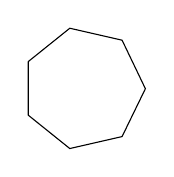
\begin{tikzpicture}[scale=0.8]
			\draw (-0.76,1.54) -- (-0.76,0.69) -- (-0.10,0.16) -- (0.73,0.35) -- (1.1,1.11) -- (0.73,1.88) -- (-0.10,2.07) -- (-0.76,1.54);
		\end{tikzpicture}\label{fig:pattern_heptagon}
	}\hfill
	\subfloat[Circle]{
		
\begin{tikzpicture}[scale=0.8]
			\draw (0,0) circle(1);
		\end{tikzpicture}\label{fig:pattern_circle}
	}\hfill
	\caption{Different laser patterns}
	\label{fig:laser_pattern}
\end{figure}

Criteria for a good pattern should contain
\begin{enumerate}
	\item Not ambiguous when interpolating lines
	\item Easy algorithm to reconstruct shape
	\item Keep orientation information\footnote{Avoid apperture problem, see section \vref{sec:apperture.problem}}
\end{enumerate}

It can be shown that amongst the patterns in figure \vref{fig:laser_pattern} that all patterns with a even number 
of vertices is prone to the apperture problem. 

\cleardoublepage{}


\chapter{Computer Vision and algorithms}

Computer vision has seen a substancial growth over the last 40 years, as camera technology became mature 
and the analysis of data became cheaper and faster. In this chapter we are going to look at the main algorithms 
that were tested and applied in the project, and give some more depth in the algorithms and mathematichs behind each of them.

\section{Thresholding}

\subsection{Naïve thresholding}

\subsection{Adaptive thresholding}


\section{Bluring}



\section{Optical flow}
Optical flow is a term that covers the apparent motion of objects, spcifically its edges and surfaces 
relative to an observer. The term was first coined for this by James Gibson in the 1940s 
to describe the visual stimulus that animals get from movement\citet{gibson50}.


\subsection{Theory}
The base of optical flow theory is based on the normal flow constraint equation in \eqref{equ:image.constraint}. In equation \eqref{equ:image.constraint}, $I$ is the intensity
at a given point at a given time. It is quite abvious that a normal optical flow problem will be of three dimension as it will include spatial coordinates in addition
to a temporal part. The deltas shown is an indefinite movement in the three dimensions.


\begin{equation}
I(x,y,t) = I(x + \Delta x, y+ \Delta y, t + \Delta t)
\label{equ:image.constraint}
\end{equation}

If the deltas in equation \eqref{equ:image.constraint} is assumed to be small, then the approximation in equation \eqref{equ:image.constraint.taylor} is valid.

\begin{equation}
I(x + \Delta x, y+ \Delta y, t + \Delta t) = I(x,y,t) + \frac{\partial I}{\partial x} \Delta x + \frac{\partial I}{\partial y} \Delta y + \frac{\partial I}{\partial t} \Delta t + \mathcal{O}(\partial^2)
\label{equ:image.constraint.taylor}
\end{equation}

Equation \eqref{equ:image.constraint.taylor} contains a higher order collection term $\mathcal{O}(\partial^2)$. This can be thought of the error in this first order taylor approximation. As
the deltas are assumed small, then the taylor expansion terms with order higher than one is negligible. 

Substituting equation \eqref{equ:image.constraint} into \eqref{equ:image.constraint.taylor} it is obvious that equation \eqref{equ:taylor.exp} must hold. 
By dividing equation \eqref{equ:taylor.exp} with the change of time we get \eqref{equ:taylor.exp.subs}, where $V_x$ and $V_y$ are the spatial velocities in the 
$x$ and $y$ direction.

\begin{align}
\frac{\partial I}{\partial x} \Delta x + \frac{\partial I}{\partial y} \Delta y + \frac{\partial I}{\partial t} \Delta t &= 0 \label{equ:taylor.exp} \\
\frac{\partial I}{\partial x} \frac{\Delta x}{\Delta t} + \frac{\partial I}{\partial y} \frac{\Delta y}{\Delta t} + \frac{\partial I}{\partial t} \frac{\Delta t}{\Delta t} &= \frac{0}{\Delta t} \notag \\
\frac{\partial I}{\partial x} V_x + \frac{\partial I}{\partial y} V_y + \frac{\partial I}{\partial t}  &= 0 \label{equ:taylor.exp.subs}
\end{align}

By defining the intensity spatial derivatives as $I_x$, $I_y$ and $I_t$, we get equation \eqref{equ:intensity.deriv}. Using the dot product on the derivatives 
leads to equation \eqref{equ:optical.flow}, which is the usual way of writing the optical flow problem.

\begin{align}
I_x V_x + I_y V_y &= -I_t \label{equ:intensity.deriv} \\
\nabla I^\top \cdot \vec{V} &= -I_t \label{equ:optical.flow}
\end{align}

Equation \eqref{equ:optical.flow} shows the big problem of optical flow problems. It is a single equation with two unknowns, and is therefore not 
solvable without adding additional constraints to the analysis. The problem is known as the aperture problem, and all of the following algorithms 
introduces some additional condition that inferes constraints to the flow problem.

\subsection{Phase correlation}
As the name of this method implies, this method uses shift and correlation in the phase plane between to frames as a measure of motion. Given that correlation is a global operation,
the method is also image global. The first step is to apply the Fourier transform to both frames, $\textbf{G}_a = \mathcal{F}\{g_a\}$ and $\textbf{G}_b = \mathcal{F}\{g_b\}$. The cross-power spectrum 
can then be calculated with equation \eqref{equ:phase.cross.power}.

\begin{equation}\label{equ:phase.cross.power}
R = \frac{\textbf{G}_a \circ \textbf{G}_b^\star}{|\textbf{G}_a \textbf{G}_b^\star|}
\end{equation}

By inverse transforming $R$, we get the normalized cross-correlation, $r = \mathcal{F}^{-1}\{R\}$, which can be though of as a 
heat map of the movement between the two frames.

There are however some drawbacks with using the phase correlation method, in addition to the global aspect. The global aspect 
inferes smooth and equal movement of all points between the frames. Also, since the Fourier transform is involved. The method has its base 
in the Fourier shift theorem, which implies that the images are assumed to have a circular shift. The case is, however, that the shift 
is more likely to be linear, and this discrepancy gives distortions in the cross-correlation.

\subsection{Lukas-Kanade}
The Lucas-Kanade method is a widely used method for providing the needed constraints to solve \eqref{equ:optical.flow}. This method assumes that 
the motion between to frames is small and more or less constant in the neighborhood of a point, known as the velocity smoothness constraint. 
This means that \eqref{equ:optical.flow} holds for all points within some window
with the point that is being considered. This means that the local velocity vector should satisfy \eqref{equ:lk.local.flow}.

\begin{align}\label{equ:lk.local.flow}
I_x(q_1)V_x + I_y(q_1)V_y	&= -I_t(q_1) \\
I_x(q_2)V_x + I_y(q_2)V_y 	&= -I_t(q_2) \notag \\
&\,\,\, \vdots \notag \\
I_x(q_N)V_x + I_y(q_N)V_y 	&= -I_t(q_N) \notag
\end{align}

Rewriting \eqref{equ:lk.local.flow} on matrix form using the normal $Av = b$ structure, we get the matrices in \eqref{equ:lk.local.flow.mat}.

\begin{equation} \label{equ:lk.local.flow.mat}
A = 
\begin{bmatrix}
	I_x(q_1) 	& I_y(q_1) \\
	I_x(q_2) 	& I_y(q_2) \\ 
	\vdots 		& \vdots \\
	I_x(q_N)	& I_y(q_N)
\end{bmatrix} \quad 
v = 
\begin{bmatrix}
V_x \\ V_y
\end{bmatrix} \quad
b = 
\begin{bmatrix}
-I_t(q_1) \\ -I_t(q_2) \\ \vdots \\ -I_t(q_N)
\end{bmatrix}
\end{equation}

The equation set in \eqref{equ:lk.local.flow.mat} is overdetermined. The Lucas-Kanade method now uses the 
least squares method to find the minimal solution to this set. The system that then must be solved usually takes the 
form of \eqref{equ:lk.local.flow.solv}.

\begin{equation}\label{equ:lk.local.flow.solv}
v = \left(A^\top A\right)^{-1} A^\top b
\end{equation}

If equation \eqref{equ:lk.local.flow.solv} is expanded back to its original matrices and using sums, we have the system in \eqref{equ:lk.local.flow.solv.full}

\begin{equation}\label{equ:lk.local.flow.solv.full}
\begin{bmatrix}
V_x \\ V_y
\end{bmatrix} = 
\begin{bmatrix}
\sum_ i{I_x^2(q_i)} 	 & \sum_i{I_x(q_i)I_y(q_i)} \\
\sum_i{I_y(q_i)I_x(q_i)} & \sum{I_y^2(q_i)}
\end{bmatrix}^{-1}
\begin{bmatrix}
-\sum_i{I_x(q_i)I_t(q_i)} \\ -\sum_i{I_y(q_i)I_t(q_i)}
\end{bmatrix}
\end{equation}

\subsection{Horch-Schunck}

\cleardoublepage


\chapter{Application of Algorithms}
In this chapter the main algorithms that were covered in chapter \ref{chp:vision} are going to 
be examined in a more practical fashion. The algorithms will 
be prototyped against the navigation scenario in a net.

As mentioned in section \vref{sec:high_def_video_analysis} all implementations done uses the open source \gls{ocv} library. This is done 
through the \gls{python} bindings made available by the project for prototyping, and through the \gls{cpp} API to see how 
the runtime of the algorithms compare. By design, \gls{python} will be slower than the \gls{cpp} versions as \gls{python} is a 
interpreted and \gls{jit} based run time. This means that the \gls{python} runtime needs to perform \gls{marshalling} which 
gives a speed impact.

\section{Optical flow algorithms}

\subsection{Flow fields}
Lucas-Kanade is the main algorithm that tries to identify optical flow by modelling the difference between two frames as a flow field. This algorithm 
is described in section \vref{sec:lukas-kanade}. 

The version of Lucas-Kanade that were implemented is based on the pyramid version of the algorithm. This makes the 
algorithm less computational expensive. The pyramid is built up based on the \verb|cv::goodFeaturesToTrack| function in the OpenCV library. 
This function uses a Canny edge detector to detect features in a frame. This makes use of the fact that edge intersections 
normally does not deform between two frames. Features that are traceable will by that argument be in the 
concave section of two or more intersecting Canny lines.

The initialization of the feature points yields the image in figure \vref{fig:lk_1}. The red circles shows 
where the Canny detector has found strong enough line intersections.

\begin{figure}[htbp]
	\centering
	\includegraphics[width=\textwidth]{lk_pyramid_1}
	\caption{Initialization point of Lucas-Kanade. Red dots show the tracking result from the Canny Edge Detector.}
	\label{fig:lk_1}
\end{figure}

The problem with finding good enough features becomes evident after some time. Figure \vref{fig:lk_2} shows the 
tracking result after \SI{1}{\second}. Since the features needs to be constant to be tracked, no new features are found as masks in the net moves 
off the screen. This is mainly rooted in the normal application of algorithms such as this. Normally, the algorithm would be used to track either a single object or 
some discrete number of objects in a stream of frames. 

Applying the Lucas-Kanade algorithm however to the net scenario yields bad results. One reason is that the track points starts to slip on the features 
that were chosen to be tracked. The reason for this is the relative uniformity of the environment, which is not something that the Lucas-Kanade algorithm 
were designed to track. This is rooted in the velocity smoothness constraint mentioned in section \ref{sec:lukas-kanade} 

\begin{figure}
	\centering
	\includegraphics[width=\textwidth]{lk_pyramid_2}
	\caption{1 second of tracking using the Lucas-Kanade algorithm with the initialization from \ref{fig:lk_1}.}
	\label{fig:lk_2}
\end{figure}

\subsection{Energy fields}

\subsubsection{Horn-Schunck}
The main algorithm that uses energy fields to model the flow between two frames is the Horn-Schunck algorithm described in section \vref{sec:horn-schunck}. This 
algorithm has been more or less replaced by the \citet{farnebackSCIA03} algorithm, as described in section \vref{sec:farneback}. 

On this background, the Horn-Schunck 
algorithm were not implemented or tested. 
This is mainly because of the statistical data presented by \citet{farnebackSCIA03} showing that the 
Farnebäck algorithm never gives a worse result than the Horn-Schunck algorithm, while proving to be 
less computational expensive.

\clearpage

\subsubsection{Farnebäck}
Farnebäck became the algorithm with a base in the theory of energy fields that were implemented. This 
is quite a new algorithm in the field of optical flow, but it has proven itself to be 
quite a robust and attractive algorithm. The implementation is based on \citet{farnebackSCIA03} by 
using the \gls{ocv} library.

The image in figure \ref{fig:farneback_1} shows the field calculated 
by the algorithm during linear translation in a realistic scenario. This means 
that even though the majority of movement found goes in the 
downward direction. A close-up view can be seen in figure \ref{fig:farneback_2}.

\begin{figure}[htbp]
	\centering
	\includegraphics[width=\textwidth]{farneback_1}
	\caption{Using \citet{farnebackSCIA03} to track movement when net is lowered. Each point is the sum of movement in the 
		rectangle which the point is in the centre of that spans to a equidistant grid over the whole image.}
	\label{fig:farneback_1}
\end{figure}

\begin{figure}[htbp]
	\centering
	\includegraphics[height=\textwidth, angle=90]{farneback_2}
	\caption{Closer look at the output from \citet{farnebackSCIA03} on a subset of masks. Almost uniform flow 
		is detected in the points where the net movement happens. Up direction is to the left in the image.}
	\label{fig:farneback_2}
\end{figure}

Since this algorithm estimates the field in a grid, it can be 
sensitive to weak references and smoothing. A example of real life conditions 
that may lead to a loss of the field in areas with low contrast is shown in 
figure \ref{fig:farneback_3}.

\begin{figure}[htbp]
	\centering
	\includegraphics[width=\textwidth]{farneback_3}
	\caption{Overview of tracking. Note good tracking in points that contains the vertical parts of the masks and the loss of tracking in 
		the lover left corner.}
	\label{fig:farneback_3}
\end{figure}

Based on how the algorithm calculates the flow, it is also obvious that the Farnebäck algorithm 
is susceptible to other foreground objects that will distort the measurement of the flow for the net. 
This is based in the local grid that this algorithm uses, and it therefore does 
not use some global measurement to detect the mean flow. These features can be seen in figure \ref{fig:farneback_dist_1} and 
\ref{fig:farneback_dist_2}.

\begin{figure}[htbp]
	\centering
	\includegraphics[height=\textwidth, angle=90]{farneback_distortion_1}
	\caption{Showing \citet{farnebackSCIA03} tracking other unwanted objects in the stream. Here some small air bubble are being tracked. 
		Upwards direction is to the left in the image.}
	\label{fig:farneback_dist_1}
\end{figure}

\begin{figure}[htbp]
	\centering
	\includegraphics[width=\textwidth]{farneback_distortion_2}
	\caption{Showing \citet{farnebackSCIA03} tracking the bottom line of the rig. Multiple big distortions.}
	\label{fig:farneback_dist_2}
\end{figure}

The hard distortions seen if figure \ref{fig:farneback_dist_1} and 
\ref{fig:farneback_dist_2} stems from the intended use 
of the algorithm. It is optimized to find either global flow when 
the image only contains background, or to track objects in the foreground. 

The Farnebäck algorithm were tested on a sample video. The movement detected by
the algorithm has been plotted in figure \vref{fig:farneback_move}. Note that 
the dimensions for the movement are related by 
some scaling factor to the real movement in the image stream.

\begin{figure}[htbp]
    \centering
    \subfloat[Result of the Farnebäck algorithm detected movement on a sample video.]
    	{\label{fig:farneback_move_1}{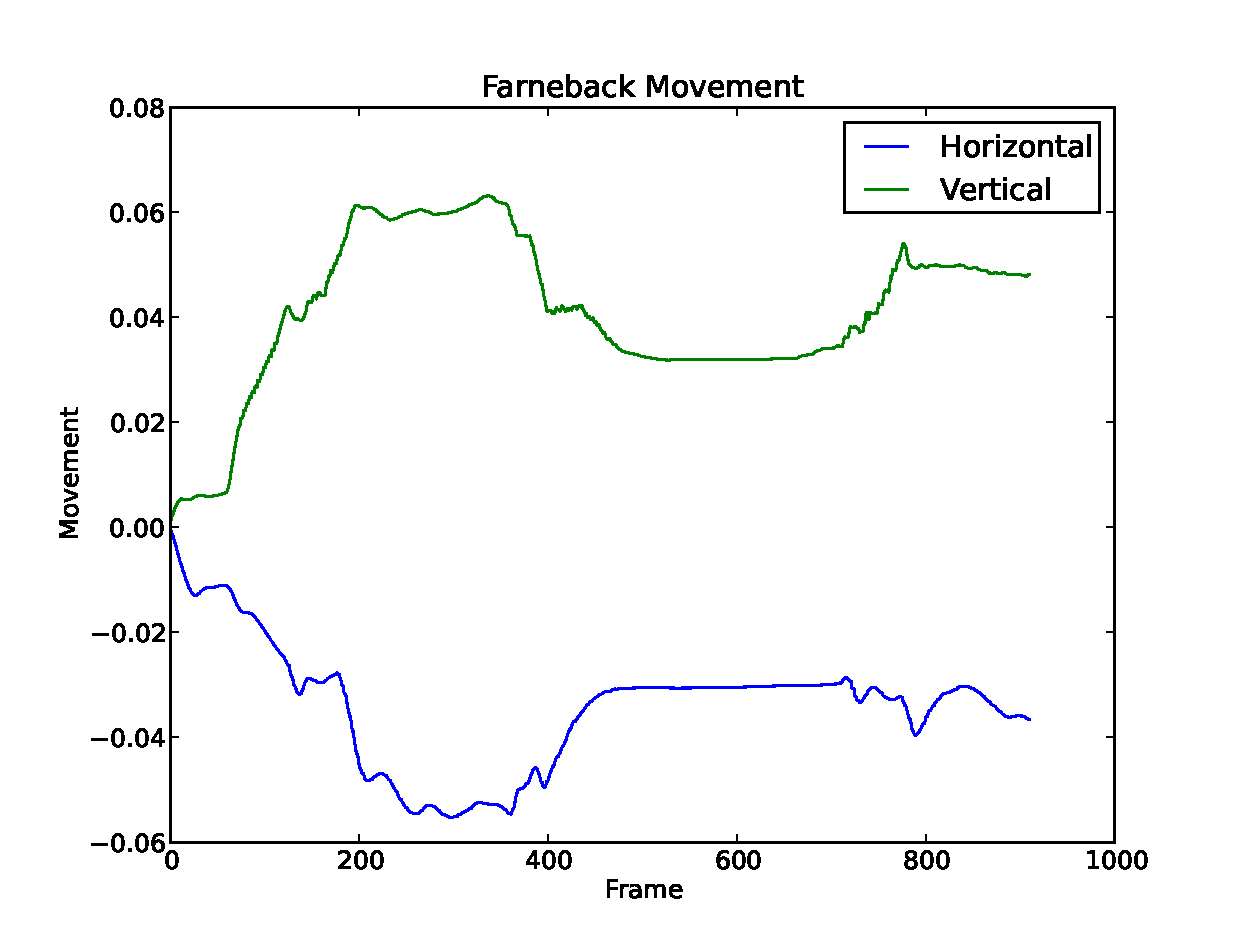
\includegraphics[width=0.8\textwidth]{farneback_move_1}}}
    \\
	\subfloat[Result of the Farnebäck algorithm detected movement on a sample video, horizontal position plotted against vertical position.]
		{\label{fig:farneback_move_2}{\includegraphics[width=0.8\textwidth]{farneback_move_2}}}
	\caption{Using the Farnebäck algorithm on a sample video. 
		Shown as position vs frame (\ref{fig:phase_run_1}) and x-position vs y-position (\ref{fig:phase_run_2}).}
	\label{fig:farneback_move}
\end{figure}

\clearpage

\subsection{Line tracing}
The use of Hough Transforms was tested by \citet{carlsen10} to detect the net and masks in the net. His trials were initially done in a 
static scenario with the net held in place by a metal frame. He showed that it was possible to find the lines describing the mask 
structure using the normal Hough Transform by setting strict parameters on the minimum distance between detected lines under those conditions.
It proved however to be much worse to get stable readings during his field test, and 

The image in figure \vref{fig:hl_1} shows the results of the normal Hough Transform on the net suspended in free water. Due to the 
movement of the net, and the folding seen in figure \ref{fig:hl_1} the transform fails to find a consistent number of lines. When  
the net starts moving up as shown in figure \ref{fig:hl_2} it seems as most of the lines that were found in figure \ref{fig:hl_1} 
is being tracked correctly. However, as the Hough Transform generates a new set of lines for each image this is not an assumption 
that generally holds. 

\begin{figure}[htbp]
	\centering
	\includegraphics[width=\textwidth]{houghlines_1}
	\caption{Initial result of the Hough Line Transform on a net at rest}
	\label{fig:hl_1}
\end{figure}

\begin{figure}[htbp]
	\centering
	\includegraphics[width=\textwidth]{houghlines_2}
	\caption{Result of the Hough Line Transform when the net is moving}
	\label{fig:hl_2}
\end{figure}

According to section \vref{sec:hough.transform.prob} the Probabilistic Hough transform would be a better choice in the
environment shown in figure \ref{fig:hl_1}. This comes from the design of the algorithm to not 
assume that lines are straight for the duration of the lines. Using the probabilistic properties from section \ref{sec:hough.transform.prob} 
the image in figure \vref{fig:hl_p_1} were obtained. This is from the same sequence as figure \ref{fig:hl_1}. The image in figure \ref{fig:hl_p_2}
is from the same sequence as figure \ref{fig:hl_2}, and shows how the probabilistic transform detects lines during movement.

\begin{figure}[htbp]
	\centering
	\includegraphics[width=\textwidth]{houghlines_probabilistic_1}
	\caption{Initial result of the Probabilistic Hough Line Transform on a net at rest}
	\label{fig:hl_p_1}
\end{figure}

\begin{figure}[htbp]
	\centering
	\includegraphics[width=\textwidth]{houghlines_probabilistic_2}
	\caption{Result of the Probabilistic Hough Line Transform when the net is moving}
	\label{fig:hl_p_2}
\end{figure}

\clearpage

\subsection{Phase correlation}
The Phase Correlation algorithm that were described in section \vref{sec:phase.correlation} were also tested. This 
is one of the older methods of finding flow, and it is mainly designed to find the linear translation between two frames.
The use of a phase plane makes the algorithm extremely resilient to noise in the image. This is in sharp contradiction 
to other algorithms that work in the spatial domain.

\begin{figure}[htbp]
    \centering
    \subfloat[Result of Phase Correlation detected movement on a sample video.]
    	{\label{fig:phase_run_1}{\includegraphics[width=0.8\textwidth]{phase_run_1}}}
    \\
	\subfloat[Result of Phase Correlation detected movement on a sample video, horizontal position plotted against vertical position.]
		{\label{fig:phase_run_2}{\includegraphics[width=0.8\textwidth]{phase_run_2}}}
	\caption{Using Phase Correlation on a sample video. 
		Shown as position vs frame (\ref{fig:phase_run_1}) and x-position vs y-position (\ref{fig:phase_run_2}).}
	\label{fig:phase_run}
\end{figure}

The output from the phase correlation algorithm is the primary detected movement between two frames, and some 
statistical data about the detected movement. This means that it is easily 
plotted as shown in figure \ref{fig:phase_run}. 

The figures in figure \ref{fig:phase_run} shows the 
same video sequence plotted in two different ways. Figure \ref{fig:phase_run_1} shows the two 
different dimensions of the video and how it is detected to move during the full duration of the stream. This gives a temporal 
view of how the movement progresses. Figure \ref{fig:phase_run_2} shows a polar plot of the same, where the horizontal and vertical 
components  This plot loses the temporal component, but it shows a trace of the 
movement of the net. 

\cleardoublepage


\chapter{System implementation}


\section{Hardware setup}

\begin{sidewaysfigure}
	\centering
	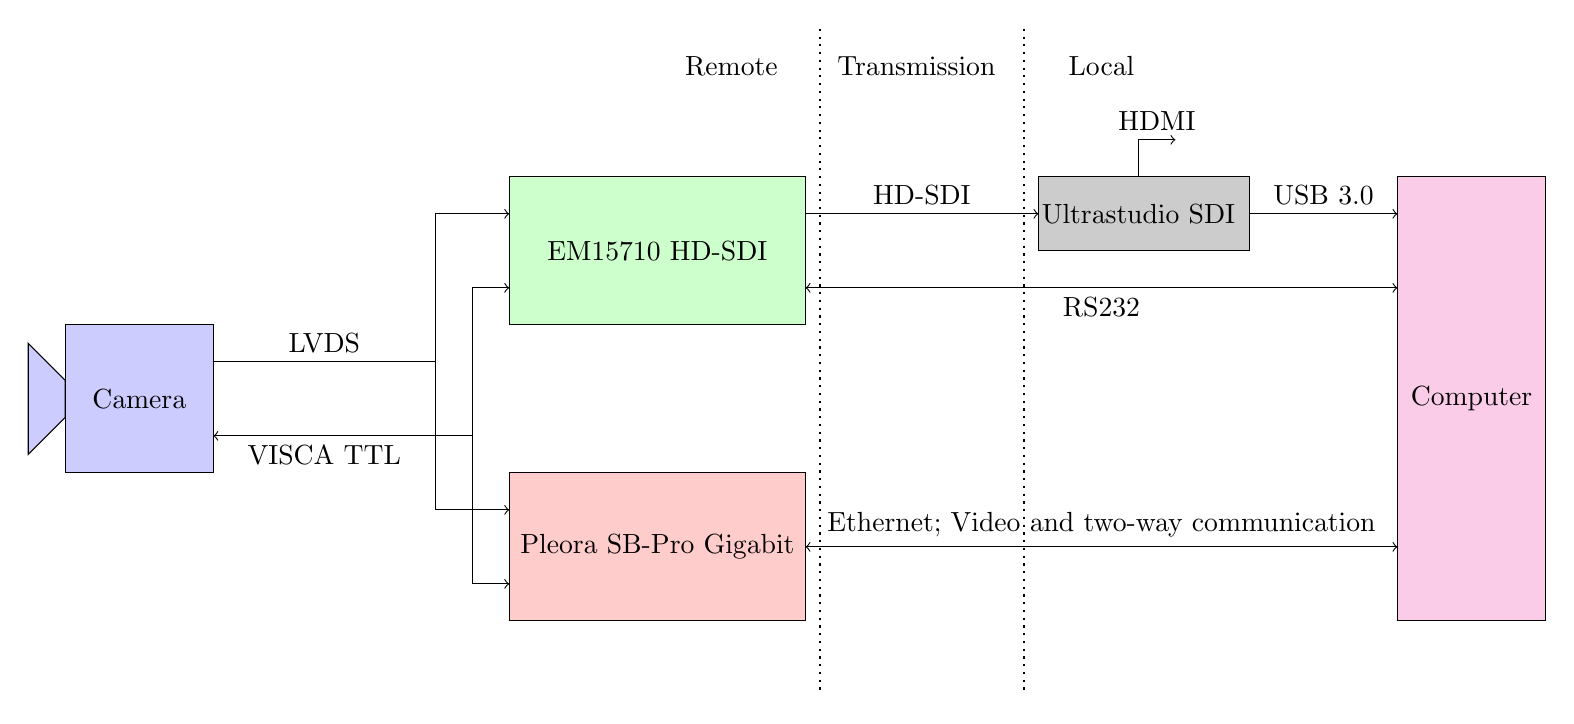
\begin{tikzpicture}[scale=0.94]
		% Camera
		\filldraw[fill=blue!20!white] (0,1) rectangle (2,-1);
		\filldraw[fill=blue!20!white] (0,0.25) -- (-0.5,0.75) -- (-0.5,-0.75) -- (0,-0.25) -- (0,0.25);
		\filldraw[fill=blue!20!white,draw=blue!20!white] (-0.1,-0.25) rectangle (0,.1,0.25);
		\node() at (1,0) {Camera};
		
		% EM
		\filldraw[fill=green!20!white] (6,1) rectangle (10,3);
		\node() at (8, 2) {EM15710 HD-SDI};
		
		% PL
		\filldraw[fill=red!20!white] (6,-1) rectangle (10,-3);
		\node() at (8, -2) {Pleora SB-Pro Gigabit};
		
		% U-SDI
		\filldraw[fill=black!20!white] (13.15,2) rectangle (16,3);
		\node() at (14.5, 2.5) {Ultrastudio SDI};
		
		% PC
		\filldraw[fill=magenta!20!white] (18,-3) rectangle (20,3);
		\node() at (19,0) {Computer};
		
		% Horiz lines
		\draw[thick,dotted] (10.2,5) -- (10.2,-4);
		\draw[thick,dotted] (12.95,5) -- (12.95,-4);
		
		% Top lines
		\node() at (9, 4.5){Remote};
		\node() at (11.5, 4.5){Transmission};
		\node() at (14, 4.5){Local};
		
		% Signal lines from camera
		\draw[] (2, 0.5) -- (5, 0.5) node [midway, above] {LVDS};
		\draw[->] (5, -0.5) -- (2, -0.5) node [midway, below] {VISCA TTL};
		
		% Signal lines to EM
		\draw[->] (5, 0.5) -- (5, 0.5) -- (5, 2.5) -- (6, 2.5);% LVDS
		\draw[->] (5, -0.5) -- (5.5, -0.5) -- (5.5, 1.5) -- (6, 1.5); % TTL
		
		% Signal lines to PL
		\draw[->] (5, 0.5) -- (5, 0.5) -- (5, -1.5) -- (6, -1.5); % LVDS
		\draw[->] (5, -0.5) -- (5.5, -0.5) -- (5.5, -2.5) -- (6, -2.5); % TTL
		
		% Signal line from EM to U-SDI
		\draw[->] (10,2.5) -- (13.15, 2.5) node [midway, above]{HD-SDI};
		
		% Signal line from U-SDI, HDMI
		\draw[->] (14.5,3) -- (14.5, 3.5) -- (15, 3.5) node [midway, above]{HDMI};
				
		% Signal line from EM to PC
		\draw[<->] (10,1.5) -- (18, 1.5) node [midway, below]{RS232}; 
		
		% Signal line from U-SDI to PC
		\draw[->] (16, 2.5) -- (18, 2.5) node [midway, above]{USB 3.0};
		
		% Signal line from PL to PC
		\draw[<->] (10,-2) -- (18, -2) node [midway, above]{Ethernet; Video and two-way communication}; 
	\end{tikzpicture}
	\caption{Schematics of the hardware}
	\label{fig:hw.schema}
\end{sidewaysfigure}
\cleardoublepage{}


\chapter{Field Tests}\label{ch:field_test}

Computer Vision algorithms can only give as good result as the source videostream that it is 
being fed. After talking a bit to \gls{sintef}, some test videos were provided by them. However, as seen in figure 
\vref{fig:sintef_not_1}, the quality leaves much to be desired. The video provided had a resolution 
of $854 \times 480$ pixels with big black box padding around it. This does not only make 
the video unsuitable for us in a computer vision algorithm, but it also means that the video 
probably is upscaled quite a bit.

Due to the poor nature of the quality of the video it was decided early on that 
a field test was needed, since we were going to use equivalent hardware as to what is available on the \gls{rov}. 

\begin{figure}[htbp]
	\centering
	\includegraphics[width=\textwidth]{sintef_not_video_1}
	\caption{Original video provided by \gls{sintef}}
	\label{fig:sintef_not_1}
\end{figure}

\section{SINTEF DVL Test}\label{sec:sintef.test}
As part of the cooperation with \gls{sintef} during the preliminary testing, we 
were asked to help with a \gls{dvl} test using a rig for controlling 
the movement of the net. As a favour for us helping out, we 
got to lend the rig at a later time when our hardware were ready to do a field test. 

During this test, we learned enough about the rig and operation of it that we should be able to operate 
it ourselves. The field test also gave some valuable information 
on how to get everything set up correctly, and what preparations which 
were needed to go through with our test.

\begin{figure}[htbp]
	\centering
	\includegraphics[width=\textwidth]{rig1}
	\caption{Field test for \gls{sintef} using \gls{dvl}}
	\label{fig:test_dvl}
\end{figure}

\section{HD Video Test}

\begin{table}[htbp]
	\centering
	\begin{tabular}{ll}
		\toprule
			Net setup 					& Description  \\
		\midrule
			Reference					& Net in static position. No forced movement. \\
			Reference with movement		& Net lowered in front of the camera. \\
			Circular hole				& Net with a circular cut-out lowered. \\
			Vertical tear				& Net with a narrow vertical tear lowered. \\
			Horizontal tear				& Net with narrow horizontal tear lowered. \\
			L-shaped tear				& Net with horizontal L-shaped tear lowered. \\
			Growth						& Net with imitation growths lowered.\\
			Double sea-cage				& Two nets laid on top of each other.\\
		\bottomrule
	\end{tabular}
	\caption{Test setup, all at \SI{1.5}{\metre}}
	\label{tbl:test_setup}
\end{table}

\begin{figure}[htbp]
    \centering
    \subfloat[Circular Hole]{\label{fig:net_hole}{\includegraphics[width=0.3\textwidth]{net_hole}}} \hfill
    \subfloat[Vertical tear]{\label{fig:net_vertical}{\includegraphics[width=0.3\textwidth]{net_vertical}}} \hfill
    \subfloat[Double net]{\label{fig:net_double}{\includegraphics[width=0.3\textwidth]{net_double}}}
    \\
	\subfloat[L-shaped tear]{\label{fig:net_L_tear}{\includegraphics[width=0.45\textwidth]{net_l}}} \hfill
	\subfloat[Horizontal tear]{\label{fig:net_horize}{\includegraphics[width=0.45\textwidth]{net_horiz}}}
	\caption{Different net configurations with holes and tears, excluding normal single net. Images collected from \citet{sletta13}.}
	\label{fig:net_configs}
\end{figure}

\begin{figure}[htbp]
	\centering
	\includegraphics[width=0.9\textwidth]{rig2}
	\caption{Field test on a sunny day in May}
	\label{fig:test_hd}
\end{figure}

The rig was configured to mimic the approximate distance to the net 
in figure \vref{fig:sintef_not_1}. We were however not able to tilt the camera to 
an angle due to environmental constraint in a anchor chain situated below the camera.
We approximated the distance between the ROV and the net in figure \vref{fig:sintef_not_1} to be 
\SI{1.5}{\metre}. This lead to a the image in figure \vref{fig:test_hd_referanse}.

\begin{figure}[htbp]
	\centering
	\includegraphics[width=\textwidth]{hd_not_all}
	\caption{View of the net from \SI{1.5}{\metre}. This is the default distance for the rig used.}
	\label{fig:test_hd_referanse}
\end{figure}

Comparing image \vref{fig:test_hd_referanse} and \vref{fig:sintef_not_1}, it seems that the 
top row of masks is approximately the same in both images. Due to the tilt of the 
camera in image \ref{fig:sintef_not_1} we get a prominent vanishing point in that image. There 
are also some growing on the net in figure \ref{fig:sintef_not_1}, which of obvious reasons does not appear 
in figure \ref{fig:test_hd_referanse}.

\begin{figure}[htbp]
	\centering
	\includegraphics[width=\textwidth]{hd_not}
	\caption{View of masks in the net at \SI{1.5}{\metre}. Digitally zoomed in post processing.}
	\label{fig:test_hd_clip}
\end{figure}

The test was done in accordance with the test patterns described in figure \vref{fig:net_configs}. 
Nets with different holes were lowered in front of the camera, left hanging for some time, and then lifted up 
again. In addition to the different nets with holes, one net without holes were also used as a 
clean reference.



\section{Video Stream and Quality}

The video collected during the test showed off the superb quality of the camera that were acquired. The camera 
deals with the low light conditions and the clear light gradient in the image. A still image of the 
test of the net that contained growth can be seen in figure \vref{fig:video_zoom_2}. 

The image in figure \ref{fig:video_zoom_2} also shows some of the issues with the underwater conditions. 
The lower right part of the image has a very different light and contrast ratio, as a halo from the 
sun can be seen. This adds complexity to the algorithms that are to be used, and can in 
worst case lead to a total loss of data points. 

The zoom level on the camera were also tested. A normal camera will struggle to keep the same colour level 
during zoom, as the light and colour changes during zoom. As seen in figure \vref{fig:video_zoom_1}, the 
software in the camera seems to deal with this in an acceptable way. Figure \ref{fig:video_zoom_1} shows
the edge of the growth region with full zoom. The details in the image is difficult to appreciate 
when it is shown as still images. For the full effect, the reader should have a look through 
the video \verb|reference_growth.mp4| that is attached to this report.

\begin{figure}[htbp]
	\centering
	\includegraphics[width=\textwidth]{video_zoom_2}
	\caption{View of masks in and growth simulation on net at \SI{1.5}{\metre}.}
	\label{fig:video_zoom_2}
\end{figure}

\begin{figure}[htbp]
	\centering
	\includegraphics[width=\textwidth]{video_zoom_1}
	\caption{Same view as in figure \ref{fig:video_zoom_2}, but using the optical zoom in the camera.}
	\label{fig:video_zoom_1}
\end{figure}



Another problem with the video stream that were discovered at a later stage, is how the camera behaves during rapid movement. 
Due to the perceived low light conditions, it seems that the camera increases the shutter speed to allow more 
light into the camera sensor. 

The shutter speed of the camera during the underwater operation seems to 
have been \SI{1/50}{\second} which caused motion blurring to be introduced. This 
causes the masks in the net to be blurred out, resembling that of a 
Gaussian filter. Back in the office, it was discovered that the camera can lock the 
shutter in different modes, allowing manual control of the shutter. The camera 
is capable of a speed of \SI{1/2}{\second} to \SI{1/10000}{\second} in 21 steps. 
The movement artefacts can be seen in figure \ref{fig:fart_ufok}.


\begin{figure}[hbp]
	\centering
	\includegraphics[width=\textwidth]{fart_ufok}
	\caption{The raw video during rapid movement}
	\label{fig:fart_ufok}
\end{figure}


\section{Software}
The software used during the field tests were mainly the software provided with the Ultrastudio unit. This capture software provided a stable connection to 
the Ultrastudio unit. It also made it possible to capture all the sequences that were done as raw video. The raw video could then be compressed on a later 
stage to ensure that the quality during tests were as close to the raw stream as possible.

\subsection{Capture constraints}

During the initial tests, it was discovered that the throughput of the capture was far greater than that the laptop were able 
to save to disk. This meant that the capture were done to ram, and push to the disk at a later stage. This meant that the length of each sequence needed to 
be quite short, as the laptop that were used would exhaust its memory in approximately 30 seconds of capture. This caused frames to 
be skipped in some of the captured files.
\cleardoublepage{}


\chapter{Discussion}

\section{Algorithms}

\subsection{Contour based tracking}


\section{Computational complexity and optimizations}
\todo{!}

\subsection{Pyramids}
\todo{!}

\subsubsection{Mimic peripheral vision}


\subsection{Filtering}
\todo{!}

\subsection{Parallel computation}

\subsection{Hardware accelerated computation}

\subsection{Quantifying bounds of aliasing and velocity}
\cleardoublepage{}

\include{conclusion}
\cleardoublepage{}

\include{further}
\cleardoublepage{}

\renewcommand*{\bibname}{References}
\bibliographystyle{plainnat}
\bibliography{bibliography}

%% Uncomment the following if you have any appendix
 \appendix
 \addtocontents{toc}{%
  \protect\vspace{1em}% 
  \protect\noindent \bfseries \appendixtocname\protect\par
  \protect\vspace{-.5em}%
 }
% \renewcommand{\chaptername}{\appendixname}
%% include below possible appendices (chapters)
% !TeX spellcheck = nb_NO

\section{Kondensatorligninger}\label{appendix:cond}
I disse avsnittene er ligningene for parallellplatekondensator, \vref{appendix:parallel}, og 
variabel kapasitanskondensatorer, \vref{appendix:var_cap} gjengitt. 
\subsection{Parallellplatekondensator}\label{appendix:parallel}
Ved å bruke definisjonen av strøm
\begin{equation}
	\frac{\mathrm{d}}{\mathrm{d}t}q(t) = i(t)
	\label{eq:i}
\end{equation}
sammen med ligning \eqref{eq:capactiance} får vi
\begin{equation}
	i(t) = \frac{\mathrm{d}}{\mathrm{d}t}\big(C(t)v(t)\big)
	\label{eq:cap_iv}
\end{equation}

Ligning \eqref{eq:cap_iv} gir en sammenheng mellom strøm gjennom en kondensator og spenning over kondensatoren. 
Det er også tydelig av ligningen at det må legges en varierende spenning 
over kondensatoren for å den skal lede. 

Ved å løse \eqref{eq:cap_iv} med hensyn på \(v(t)\) får vi
\begin{equation}
	v(t) = \frac{1}{C} \int^t_{-\infty}{i(\tau)\,\mathrm{d}\tau}
	\label{eq:cap_v}
\end{equation}
som er standardlikningen for spenningsutvikling over en kondensator ved en variabel strøm, gitt at $C$ er konstant. 

\subsection{Variabel kapasitansligning}\label{appendix:var_cap}
Antagelsen i appendiks \vref{appendix:parallel} er feil, da vi i denne oppgaven 
er ute etter å måle akkurat den \(C\) som varierer med tid, \(C(t)\). 
Om vi bruker definisjonen for \(i(t)\) fra ligning \eqref{eq:i} sammen 
med \eqref{eq:cap_iv}, får vi
\begin{align}
	i(t)  
	&= \frac{\mathrm{d}}{\mathrm{d}t} \big( C(t)v(t) \big)\label{eq:i.3}\\
	&= v(t)\frac{\mathrm{d}}{\mathrm{d}t}C(t) + C(t)\frac{\mathrm{d}}{\mathrm{d}t}v(t) \label{eq:i.4}
\end{align}

Som vi ser av ligning \eqref{eq:i.3} er det umulig å løse dette problemet eksplisitt med tanke på \(C(t)\) 
uten å gjøre antagelse om \(v(t)\) eller \(i(t)\).

Resultatet i ligning \eqref{eq:i.4} er hovedgrunnen til at det ikke er 
mulig å finne absoluttverdier i denne oppgaven.

\section{Enkel oppladningstidmåling}\label{appendix:oppladning}
Som et enkelt eksempel på hvordan er kapasitiv måling kan gjøres, er eksemplet under tatt med. 


En enkel algoritme i pseudokode er også gjengitt. 

\begin{center}
	\begin{circuitikz} \draw
	(0,0) node[anchor=east]{Drivpinne}
		to[short, o-*] (1,0)
		to[R, l=, *-*] (1,2)
	(0,2) node[anchor=east]{Sensorpinne}
		to[short, o-*] (1,2)
		to[C,l=Miljø, *-] (3,2)
		to[short] (3,1) node[ground]{}
	;\end{circuitikz}
\end{center}


%\begin{verbatim}[H]
%\SetAlgoLined
%\KwResult{teller $\propto$ ladetid}
%Initialiser\;
%Set drivpinne høy\;
%\While{sensorpinne ikke høy}{
%	inkrementer teller\;
%}
%\eIf{teller > 0}{
%	resultat = teller\;
%}{
%	feil\;
%}
%\end{verbatim}

Algoritmen over vil gi et tall som er proporsjonalt med antall sykler som er gjort før 
sensorpinnen er kommet opp på logisk 1 ($\approx \frac{V_{dd}}{2}$). Dette er derfor en ''single slope'' måling.

\section{Ladningsoverføring}\label{appendix:mutualcapacitance}
I denne oppgaven er QMatrix\texttrademark fra Atmel valgt som implementasjon av ladningsoverføringsmåling. Atmel utgir dokumentasjon \citet{qtan0079} for de forskjellige teknologiene 
som benyttes og kodebiblioteker for integrasjon i prosjekter.

Den teknologien som er brukt her har sin rot i algoritmen i appendiks \vref{appendix:oppladning}. Det er riktignok en mer komplisert utgave, der hele 
lesesyklusen er vist i appendiks \vref{appendix:mutualcapacitance.4} og i figur \vref{fig:cycle}. En nærmere gjennomgang av 
QMatrix er tilgjengelig i \citet{quantum2006}[QMatrix Technology Whitepaper].

Figur \vref{fig:qmatrix} viser hvordan QMatrix teknologien virker på en pekeflate, som er den primære bruken for QMatrix. 

\begin{figure}[htbp]
	\centering
	\includegraphics[width=0.8\textwidth]{img/qmatrix}
	\caption{QMatrix, hentet fra \citet{quantum2006}}
	\label{fig:qmatrix}
\end{figure}


\clearpage
\subsection{Krets}\label{appendix:mutualcapacitance.circuit}

I figur \vref{fig:chargetransfer} er kretsskjemaet som er brukt i denne oppgaven. Dette skjemaet viser kun 4 punkter, men det er en enkel utvidelse å 
bruke denne kretsen på \(n+m\) punkter som forsøkt vist med subskriptene på linjene.

\begin{figure}[H]
\begin{center}
	\begin{circuitikz}[scale=1.1]
	\draw[dashed,rounded corners] (7.5,9.5) rectangle (5.5,7.5);
	\foreach \x in {8,9} {
		\foreach \y in {6,7} {
			\node[circle,draw] at (\y,\x) {};
		}
	}
	\node[above] at (7.5,9.5) {Membran fra figur \vref{fig:sampl_point}};
	
	\draw
	(0,0) node[anchor=east]{SMP}
		to[short, o-*] (1,0)
		to[R, l=$\text{RYB}_0$] (1,2)
		to[short] (1,3)
		to[short] (0,3)
	(0,3) node[anchor=east]{$\text{YB}_0$}
		to[short, o-*] (1,3)
		to[short] (1,4)
		to[C, l=$\text{CS}_0$] (1,5)
	(0,2) node[anchor=east]{$\text{YB}_m$}
		to[short, o-*] (3,2)
		to[R, l=$\text{RYB}_m$] (3,0)
		to[short] (1,0)
	(3,2) node{}
		to[short] (3,4)
		to[C, l=$\text{CS}_m$] (3,5)
	(0,6) node[anchor=east]{$\text{YA}_m$}
		to[short,o-*] (3,6)
		to[short] (3,5)
	(0,7) node[anchor=east]{$\text{YA}_0$}
		to[short,o-*] (1,7)
		to[short] (1,5)
	(3,6) node{}
		to[R, l=$\text{RY}_m$] (5,6)
		to[short] (7,6)
		to[short] (7,9)
	(1,7) node{} 
		to[short] (3,7)
		to[R, l=$\text{RY}_0$] (5,7)
		to[short] (6,7)
		to[short] (6,9)
	(0,8) node[anchor=east]{$\text{X}_n$}
		to[short, o-*] (3,8)
		to[R, l=$\text{RX}_n$] (5,8)
		to[short] (7,8)
	(0,9) node[anchor=east]{$\text{X}_0$}
			to[short, o-*] (3,9)
			to[R, l=$\text{RX}_0$] (5,9)
			to[short] (7,9)
	;\end{circuitikz}
\end{center}
\caption{Ladningsoverføringskrets}
\label{fig:chargetransfer}
\end{figure}

\pagebreak
Forkortelser og linjer brukt i figur \vref{fig:chargetransfer} er beskrevet under.

\begin{description}
	\item[$\text{X}_n$] Drivlinjene. Kobles til en I/O port.
	\item[$\text{YA}_m$] I/O Porter. Her vil spenningen over $\text{CS}_m$ legge seg. Brukes for å lade ut $\text{CS}_m$.
	\item[$\text{YB}_m$] ADC porter. Måler utviklingen av oppladningen over $\text{CS}_m$.
	\item[SMP] Generel I/O port. Pulser tilbake over $\text{CS}_m$. Dette setter opp en negativ spenning som driver $\text{CS}_m$ tilbake mot 0
	\item[$\text{RYB}_m$] Pull-down resistor 
	\item[$\text{CS}_m$] Samplingkondensator. Lades opp av $\text{X}_m$
\end{description}

Den kretsen som er skissert i figur \vref{fig:chargetransfer} vil ha flere ekvivalenter ettersom hvilken del av oppladningssykelen som kretsen
er i. Disse ekvivalentene er gjennomgått i appendiks \vref{appendix:mutualcapacitance.1}, \vref{appendix:mutualcapacitance.2} og \vref{appendix:mutualcapacitance.3}.

\vfill

\pagebreak
\subsection{Ekvivalenskrets under oppladning}\label{appendix:mutualcapacitance.1}
\begin{figure}[H]
\begin{center}
	\begin{circuitikz}[scale=1.3]
	\draw[dashed,rounded corners] (7.5,9.5) rectangle (5.5,7.5);
		\foreach \x in {8,9} {
			\foreach \y in {6,7} {
				\node[circle,draw] at (\y,\x) {};
			}
		}
		\node[above] at (7.5,9.5) {Membran fra figur \vref{fig:sampl_point}};
		
	
	\draw
	(0,0) node[anchor=east]{SMP}
		to[short, o-*] (1,0)
		to[R, l=$\text{RYB}_0$] (1,2)
		to[short] (1,3)
		to[short] (1,4)
		to[C, l=$\text{CS}_0$] (1,5)
	(0,-1) node[ground]{}
		to[short](0,0)
	%(0,3) node[anchor=east]{$\text{YB}_0$}
	%	to[short, o-*] (1,3)
	%	to[short] (1,4)
	%	to[C, l=$\text{CS}_0$] (1,5)
	%(0,2) node[anchor=east]{$\text{YB}_m$}
	%	to[short, o-*] (3,2)
	%	to[R, l=$\text{RYB}_m$] (3,0)
	%	to[short] (1,0)
	(3,2) node{}
		to[R, l=$\text{RYB}_m$] (3,0)
		to[short] (1,0)
	(3,2) node{}
		to[short] (3,4)
		to[C, l=$\text{CS}_m$] (3,5)
	%(0,6) node[anchor=east]{$\text{YA}_m$}
	%	to[short,o-*] (3,6)
	%	to[short] (3,5)
	%(0,7) node[anchor=east]{$\text{YA}_0$}
	%	to[short,o-*] (1,7)
	%	to[short] (1,5)
	(3,6) node{} 
		to[short] (3,5)
	(1,7) node{}
		to[short] (1,5)
		
	(3,6) node{}
		to[R, l=$\text{RY}_m$] (5,6)
		to[short] (7,6)
		to[short] (7,9)
	(1,7) node{} 
		to[short] (3,7)
		to[R, l=$\text{RY}_0$] (5,7)
		to[short] (6,7)
		to[short] (6,9)
	(0,8) node[anchor=east]{$\text{X}_n$}
		to[short, o-*] (3,8)
		to[R, l=$\text{RX}_n$] (5,8)
		to[short] (7,8)
	(0,9) node[anchor=east]{$\text{X}_0$}
			to[short, o-*] (3,9)
			to[R, l=$\text{RX}_0$] (5,9)
			to[short] (7,9)
	;\end{circuitikz}
\end{center}
\caption{Ekvivalenskrets under oppladning}
\label{fig:chargetransfer_in}
\end{figure}

\pagebreak
\subsection{Ekvivalenskrets under motladning}\label{appendix:mutualcapacitance.2}
\begin{figure}[H]
\begin{center}
	\begin{circuitikz}[scale=1.8] \draw
	(0,5.5) node[ground]{}
		to[short] (0,6)
		to[short] (0,7)
	(0,0) node[anchor=east]{SMP}
		to[short, o-*] (1,0)
		to[R, l=$\text{RYB}_0$] (1,2)
		to[short] (1,3)
		to[short] (1,4)
		to[C, l=$\text{CS}_0$] (1,5)
	(0,3) node[anchor=east]{$\text{YB}_0$}
		to[short, o-*] (1,3)
		to[short] (1,4)
	(0,2) node[anchor=east]{$\text{YB}_m$}
		to[short, o-*] (3,2) 
	(3,2) node{}
		to[R, l=$\text{RYB}_m$] (3,0)
		to[short] (1,0)
	(3,2) node{}
		to[short] (3,4)
		to[C, l=$\text{CS}_m$] (3,5)
	(0,6) node[anchor=east]{$\text{YA}_m$}
		to[buffer] (3,6)
		to[short] (3,5)
	(0,7) node[anchor=east]{$\text{YA}_0$}
		to[short,o-*] (1,7)
		to[short] (1,5)
	(3,6) node{} 
		to[short] (3,5)
	(1,7) node{}
		to[short] (1,5)
		
	%(3,6) node{}
	%	to[R, l=$\text{RY}_m$] (5,6)
	%	to[short] (7,6)
	%	to[short] (7,9)
	%(1,7) node{} 
	%	to[short] (3,7)
	%	to[R, l=$\text{RY}_0$] (5,7)
	%	to[short] (6,7)
	%	to[short] (6,9)
	%(0,8) node[anchor=east]{$\text{X}_n$}
	%	to[short, o-*] (3,8)
	%	to[R, l=$\text{RX}_n$] (5,8)
	%	to[short] (7,8)
	%(0,9) node[anchor=east]{$\text{X}_0$}
	%		to[short, o-*] (3,9)
	%		to[R, l=$\text{RX}_0$] (5,9)
	%		to[short] (7,9)
	;\end{circuitikz}
\end{center}
\caption{Ekvivalenskrets under motladning}
\label{fig:chargetransfer_out}
\end{figure}



\pagebreak
\subsection{Ekvivalenskrets under utladning}\label{appendix:mutualcapacitance.3}
\begin{figure}[H]
\begin{center}
	\begin{circuitikz}[scale=1.5] \draw
	(0,5.5) node[ground]{}
		to[short] (0,6)
		to[short] (0,7)
	(0,0) node[anchor=east]{SMP}
		to[short, o-*] (1,0)
		to[R, l=$\text{RYB}_0$] (1,2)
		to[short] (1,3)
		to[short] (1,4)
		to[C, l=$\text{CS}_0$] (1,5)
	(0,3) node[anchor=east]{$\text{YB}_0$}
		to[short, o-*] (1,3)
		to[short] (1,4)
	(0,2) node[anchor=east]{$\text{YB}_m$}
		to[short, o-*] (3,2) 
	(3,2) node{}
		to[R, l=$\text{RYB}_m$] (3,0)
		to[short] (1,0)
	(3,2) node{}
		to[short] (3,4)
		to[C, l=$\text{CS}_m$] (3,5)
	(0,6) node[anchor=east]{$\text{YA}_m$}
		to[buffer] (3,6)
		to[short] (3,5)
	(0,7) node[anchor=east]{$\text{YA}_0$}
		to[short,o-*] (1,7)
		to[short] (1,5)
	(3,6) node{} 
		to[short] (3,5)
	(1,7) node{}
		to[short] (1,5)
	(0,-1) node[ground]{}
		to[short](0,0)
	%(3,6) node{}
	%	to[R, l=$\text{RY}_m$] (5,6)
	%	to[short] (7,6)
	%	to[short] (7,9)
	%(1,7) node{} 
	%	to[short] (3,7)
	%	to[R, l=$\text{RY}_0$] (5,7)
	%	to[short] (6,7)
	%	to[short] (6,9)
	%(0,8) node[anchor=east]{$\text{X}_n$}
	%	to[short, o-*] (3,8)
	%	to[R, l=$\text{RX}_n$] (5,8)
	%	to[short] (7,8)
	%(0,9) node[anchor=east]{$\text{X}_0$}
	%		to[short, o-*] (3,9)
	%		to[R, l=$\text{RX}_0$] (5,9)
	%		to[short] (7,9)
	;\end{circuitikz}
\end{center}
\caption{Ekvivalenskrets under utladning}
\label{fig:chargetransfer_reset}
\end{figure}

\pagebreak
\section{Ladesykel over \texorpdfstring{$\text{CS}_m$}{Cs}}\label{appendix:mutualcapacitance.4}


\begin{sidewaysfigure}
\begin{figure}[H]
\begin{center}
\begin{tikzpicture}[xscale=15]
	%\draw[help lines,step=0.1] (0,-8) grid (1,7);
	\draw [->, help lines] (0,-7) -- (0,6);
	\draw [->, help lines] (0,0) -- (1,0);
	\draw[rounded corners] (0,0) -- (0.04,1) -- (0.08,1) -- (0.12,2) -- (0.16,2) -- (0.20,3) -- (0.24,3) -- (0.28,4) -- (0.32,4) -- (0.36,5) -- (0.4,5) -- (0.44,4) -- (0.48,4) -- (0.52,3) -- (0.56,3) -- 
		(0.6,2) -- (0.64,2) -- (0.68,1) -- (0.72,1) -- (0.76,0) -- (0.80,0) -- (0.84,-1) -- (0.88,-1) -- (0.92,-2) -- (0.96,-2) -- (1,0);
	\draw[thin,dashed] (0.38,-7) -- (0.38,6);
	\node[above] at (0.36,6) {1. fase ferdig};
	\node[right] at (0.4,5) {Start utladning};
	\draw[thin,dashed] (0.78,-7) -- (0.78,6);
	\node[above] at (0.76,6) {2. fase ferdig};
	\draw[thin,dashed] (0.94,-7) -- (0.94,6);
	\node[above,align=center] at (0.94,6) {3. fase ferdig};
	
	\node[left] at (0,0) {$V_{\text{CS}_m}$};
	\node[left] at (0,-3) {$\text{X}_n$};
	\node[left] at (0,-5) {SMP};
	\node[left] at (0,-7) {$\text{YA}_m$};
	
	\draw[<->] (0.15,3) -- (0.15,4);
	\draw[dashed] (0.2,3) -- (0.15,3);
	\draw[dashed] (0.29,4) -- (0.15,4);
	\node[left] at (0.15,3.5) {$v_\delta$};
	
	\draw[<->]  (0.52,-2.5) -- (0.56,-2.5);
	\draw[dashed] (0.52,-4) -- (0.52,-2.5);
	\draw[dashed] (0.56,-4) -- (0.56,-2.5);
	\node[above] at (0.54,-2.5) {ADC};
	
	\draw [->, help lines] (0,-3) -- (1,-3);
	\draw (0,-2) -- (0.04,-2) -- (0.04,-3) -- (0.08,-3) -- (0.08,-2) -- (0.12,-2) -- (0.12,-3) -- (0.16,-3) -- (0.16,-2) -- (0.2,-2) -- (0.2,-3) -- (0.24,-3) -- (0.24,-2) -- (0.28,-2) -- (0.28,-3) -- 
		(0.32,-3) -- (0.32,-2) -- (0.36,-2) -- (0.36,-3);
	
	\draw [->, help lines] (0,-5) -- (1,-5);
	\draw (0.4,-5) -- (0.4,-4) -- (0.44,-4) -- (0.44,-5) -- (0.48,-5) -- (0.48,-4) -- (0.52,-4) -- (0.52,-5) -- (0.56,-5) -- (0.56,-4) -- (0.60,-4) -- (0.60,-5) -- (0.64,-5) -- (0.64,-4) -- (0.68,-4) -- 
		(0.68,-5) -- (0.72,-5) -- (0.72, -4) -- (0.76,-4) -- (0.76,-5) -- (0.80,-5) -- (0.80,-4) -- (0.84,-4) -- (0.84,-5) -- (0.88,-5) -- (0.88,-4) -- (0.92,-4) -- (0.92,-5);
		
	\draw [->, help lines] (0,-7) -- (1,-7);
\end{tikzpicture}
\end{center}
\caption{Skjematisk tegning av ladesykel over $\text{CS}_m$}
\label{fig:cycle}
\end{figure}
\end{sidewaysfigure}

Figur \vref{fig:cycle} gjengir en full lesesyklus for oppsettet. 

\subsection{Fase 1}
I den første delen av figur \vref{fig:cycle} fungerer kretsen som vist i figur \vref{fig:chargetransfer_in} i appendiks \vref{appendix:mutualcapacitance.1}.

Her blir \(\text{X}_n\) brukt til å øke spenningen over \(\text{CS}_m\). Avhengig av avstanden mellom elektrodene så vil \(v_\delta\) bli større eller mindre, og 
vil dermed endre høyden på pyramiden, da det er et fast antall pulser på \(\text{X}_n\) i denne delen.

\subsection{Fase 2}\label{appendix:down}
I den andre delen av figur \vref{fig:cycle} fungerer kretsen som vist i figur \vref{fig:chargetransfer_out} i appendiks \vref{appendix:mutualcapacitance.2}. 

Her blir porten merket SMP  brukt til å lade alle kondensatorene ut. Mellom hver puls på SMP brukes ADC funksjonaliteten i mikrokontrolleren til å 
måle spenningen som ligger over alle kondensatorene. Om denne går under nullpotensialet vil antall pulser som er brukt i denne delen være et mål 
på hvor mye spenning som ble lagt over kondensatoren. Dette er en klassisk dobbelthelningsmåling\footnote{dual-slope}, som brukes da målingene blir mindre støyutsatt, og 
fysiske endringer med kondensatorene kan motvirkes til en viss grad.

\subsection{Fase 3}
I den tredje delen av figur \vref{fig:cycle} fungerer kretsen som vist i figur \vref{fig:chargetransfer_reset} i appendiks \vref{appendix:mutualcapacitance.3}.

Etter nedladningsdelen i \vref{appendix:down} vil mest sannsynlig flere av kondensatorene ha en negativ spenning, og de må derfor settes tilbake 
til et kjent nullpotensiale slik at oppladningssyklusen begynner fra et kjent spenning.


\end{document} 
